\pdfminorversion=7%
\documentclass[aspectratio=169,mathserif,notheorems]{beamer}%
%
\xdef\bookbaseDir{../../bookbase}%
\xdef\sharedDir{../../shared}%
\RequirePackage{\bookbaseDir/styles/slides}%
\RequirePackage{\sharedDir/styles/styles}%
%
\gdef\searchSpace{\ensuremath{\mathbb{X}}}%
\gdef\sespel{\ensuremath{x}}%
\gdef\opti#1{\ensuremath{#1^{\star}}}%
%
%% Print an algorithm box around something.
\protected\gdef\algobox#1#2{\resizebox{#1\paperwidth}{!}{%
\bgroup%
\fboxsep=0pt%
\fboxrule=2pt%
\mbox{\fcolorbox{white}{white}{\bgroup%
\fboxsep=2pt%
\fboxrule=2pt%
\mbox{\fcolorbox{hfuu-red!80}{hfuu-orange!60}{%
\mbox{#2}%
}}\egroup%
}}%
\egroup}}%
%
\definecolor{fOneColor}{HTML}{C00000}%
\definecolor{fTwoColor}{HTML}{0070c0}%
\definecolor{fThreeColor}{HTML}{385723}%
\definecolor{fFourColor}{HTML}{7030a0}%
\definecolor{fFiveColor}{HTML}{0000ff}%
\definecolor{fSixColor}{HTML}{00b050}%
\definecolor{fSevenColor}{HTML}{de4e00}%
%
\protected\gdef\fn#1{%
{\bgroup{%
\ifcase#1\relax\or%
\color{fOneColor}\or%
\color{fTwoColor}\or%
\color{fThreeColor}\or%
\color{fFourColor}\or%
\color{fFiveColor}\or%
\color{fSixColor}\else%
\color{fSevenColor}\fi%
\ensuremath{f_{#1}}
}\egroup}%
}%
%
%
\title{Frequency Fitness Assignment}%
%
\begin{document}%
\startPresentation%
%
\section{Introduction}%
%
\begin{frame}[t]%
\frametitle{Introduction to Optimization}%
\begin{itemize}%
\item Optimization means finding superlatives.%
\item<2-> Find the \alert{fastest} way to get from Hefei to Beijing.%
%\item<3-> Find the \alert{shortest} route through $n$~cities.%
\item<3-> Design an airplane wing with the \alert{least} aerodynamic drag.%
\item<4-> Set the pricing for these apples such that we can get the \alert{largest} revenue when selling them.%
\item<5-> Place all these chips on a circuit board so that they occupy the \alert{smallest} area while we can still properly connect and cool them.%
%\item<6-> Find the \alert{cheapest} way to transport these goods from Hefei to Wellington.%
\item<6-> Find a strategy to manage the power of the nodes in this sensor network so that full coverage is guaranteed for the \alert{longest} possible duration.%
\item<7-> And so on.%
\end{itemize}%
\locateGraphic{1}{width=0.85\paperwidth}{\sharedDir/graphics/optimization_superlatives/optimization_superlatives}{0.075}{0.2}%
\locateGraphic{2-}{width=0.35\paperwidth}{\sharedDir/graphics/optimization_superlatives/optimization_superlatives}{0.63}{0.01}%
\end{frame}%
%
\begin{frame}[t]%
\frametitle{Views on Optimization}%
\begin{itemize}%
\only<-1>{\item There are two ways to look at optimization.}%
\only<-2>{\item<2-> The economic view.}%
\item<3-> The mathematical view.%
\end{itemize}%
\locateGraphic{2}{width=0.75\paperwidth}{\sharedDir/graphics/optimization_views/optimization_views_1}{0.125}{0.3}%
\locateGraphic{3}{width=0.75\paperwidth}{\sharedDir/graphics/optimization_views/optimization_views_2}{0.125}{0.3}%
\end{frame}%
%
\begin{frame}%
\frametitle{Example: Traveling Salesperson Problem}%
\parbox{0.373\paperwidth}{%
\begin{itemize}%
%
\item In the \glsFull{optTSP}\cite{ABCC2006TTSPACS,LLRKS1985TTSPAGTOCO}, the goal is to find the shortest round-trip tour through a set of $n$~cities.%
%
\item<2-> The search space \searchSpace\ thus is the set of all possible round-trip tours through these $n$~cities, usually specified as permutations of the first $n$~natural numbers.%
%
\item<3-> The objective function~$f:\searchSpace\mapsto\realNumbers$, subject to minimization, is the length of the tour.%
%
\item<4-> The optimal solution~$\opti{\sespel}\in\searchSpace$ is the shortest possible tour.%
%
\end{itemize}%
}%
%
\locateGraphic{-3}{width=0.525\paperwidth}{\sharedDir/graphics/tsp_china/tsp_china}{0.44}{0.15}%
\locateGraphic{4-}{width=0.525\paperwidth}{\sharedDir/graphics/tsp_china/tsp_china_solution}{0.44}{0.15}%
%
\end{frame}%
%
\begin{frame}%
\frametitle{Example: Maximum Satisfiability Problem}%
\parbox{0.42\paperwidth}{%
\begin{itemize}%
%
\item The goal of the \glsFull{optMaxSAT}\cite{HS2004SLSFAA,C1971TCOTPP} problem is to find a setting of \textcolor<2>{red}{$n$~variables} that makes a Boolean formula~$F$ become True. %
The variables appear directly or \textcolor<3>{violet}{negated} in \textcolor<4>{blue}{$m$~OR\nobreakdashes-clauses}, whose results flow into \textcolor<5>{green!40!black}{one AND\nobreakdashes-clause}.%
%
\item<6-> \searchSpace\ is the set of all possible bit strings of length~$n$.%
%
\item<7-> The objective function~$f:\searchSpace\mapsto\realNumbers$ is the number of unsatisfied OR\nobreakdashes-clauses.%
%
\item<8-> The optimum~$\opti{\sespel}\in\searchSpace$ has $f(\opti{\sespel})=0$, i.e., all clauses satisfied, i.e., $F(\opti{\sespel})=\textnormal{True}$.%
%
\end{itemize}%
}%
%
\locateGraphic{-1,6-}{width=0.5\paperwidth}{\sharedDir/graphics/sat/sat_plain}{0.47}{0.3}%
\locateGraphic{2}{width=0.5\paperwidth}{\sharedDir/graphics/sat/sat_variables}{0.47}{0.3}%
\locateGraphic{3}{width=0.5\paperwidth}{\sharedDir/graphics/sat/sat_negated}{0.47}{0.3}%
\locateGraphic{4}{width=0.5\paperwidth}{\sharedDir/graphics/sat/sat_clauses}{0.47}{0.3}%
\locateGraphic{5}{width=0.5\paperwidth}{\sharedDir/graphics/sat/sat_and}{0.47}{0.3}%
%
\end{frame}%
%
\begin{frame}[t]%
\frametitle{Example: Bin Packing Problem}%
\begin{itemize}%
\item The goal of the Bin Packing Problem is to pack $n$~objects, each having a specific size, into as few bins~(also of a given size) as possible\cite{ZLWvdBTW2024RLSOT2RBPPWIR,ZWvdBTLTW2024RLSFTDBPAANRFFFA}.%
\item<2-> The \searchSpace\ comprises all possible packing orders of the $n$~objects.%
\item<3-> The objective function~$f$ is the number of bins needed by a given packing order.%
\item<4-> The optimum~$\opti{\sespel}$ is the packing order requiring the fewest bins.%
\end{itemize}%
\locateGraphic{}{width=0.85\paperwidth}{\sharedDir/graphics/bin_packing/bin_packing}{0.075}{0.5}%
\end{frame}%
%
\begin{frame}[t]%
\frametitle{Optimization is Hard}%
\begin{itemize}%
%
\item Finding the globally optimal solution~\opti{\sespel} from the set of all possible solutions~\searchSpace\ is often an \npHard\ problem.%
%
\item<2-> Currently, there is no algorithm that can \alert{guarantee} to find the optimal solution of \alert{every instance} of a given \npHard\ problem in a runtime that is not longer than polynomial in the size of the problem~(i.e., existing algorithms may need exponential runtime in the \alert{worst case}).%
%
\item<4-> In other words, if we want to guarantee to find the best possible solution~\opti{\sespel} for all possible instances of a problem, we often cannot really be much faster than testing all possible candidate solutions~$\sespel\in\searchSpace$ in the \alert{worst case}.%
%
\end{itemize}%
%
\locateGraphic{3}{width=0.65\paperwidth}{\sharedDir/graphics/function_growth/function_growth}{0.175}{0.44}%
%
\end{frame}%
%
\section{Metaheuristic Optimization}%
%
\begin{frame}%
\frametitle{Metaheuristic Optimization}%
\parbox{0.42\paperwidth}{%
\begin{itemize}%
%
\item Because of this hardness of optimization, metaheuristic algorithms that follow the Trial-and-Error idea of iterative improvement have emerged.%
\item<2-> They drop the guarantee to find the optimal solution.%
\item<3-> They try to find good solutions within a feasible runtime.%
\item<4-> They (usually) start with random solutions.%
\item<5-> And then roughly follow this cycle.%
%
\end{itemize}%
}%
%
\locateGraphic{4}{width=0.5\paperwidth}{\sharedDir/graphics/metaheuristic_cycle/metaheuristic_cycle_01}{0.47}{0.3}%
%
\locateGraphic{5}{width=0.5\paperwidth}{\sharedDir/graphics/metaheuristic_cycle/metaheuristic_cycle_02}{0.47}{0.3}%
%
\locateGraphic{6}{width=0.5\paperwidth}{\sharedDir/graphics/metaheuristic_cycle/metaheuristic_cycle_03}{0.47}{0.3}%
%
\locateGraphic{7}{width=0.5\paperwidth}{\sharedDir/graphics/metaheuristic_cycle/metaheuristic_cycle_04}{0.47}{0.3}%
%
\locateGraphic{8}{width=0.5\paperwidth}{\sharedDir/graphics/metaheuristic_cycle/metaheuristic_cycle_05}{0.47}{0.3}%
%
\locateGraphic{9}{width=0.5\paperwidth}{\sharedDir/graphics/metaheuristic_cycle/metaheuristic_cycle_06}{0.47}{0.3}%
%
\locateGraphic{10}{width=0.5\paperwidth}{\sharedDir/graphics/metaheuristic_cycle/metaheuristic_cycle_07}{0.47}{0.3}%
%
\end{frame}%
%
\begin{frame}[t]%
\frametitle{The $(1+1)$~EA and RLS}%
\begin{itemize}%
\item Local search with $|S_i|=|N_i|=1$ is the simplest realization of the metaheuristic idea.%
\item<2-> \GlsFull{algoRLS} and the \glsFull{algoEAopo} work according the same pattern~(and differ only in their unary search operator~$\mathop{move}$)\cite{DJW2002OTAOTOPOEA,CPD2018TAMPARAOEA}.%
\item<8-> They accept the new solution if it is better or equally good compared to the current solution.%
\end{itemize}%
%
%
\locate{2}{%
\algobox{0.75}{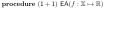
\includegraphics[width=0.75\paperwidth]{\sharedDir/graphics/metaheuristic_algorithms/opoea/opoea_1}}%
}{0.125}{0.445}%
%
\locate{3}{%
\algobox{0.75}{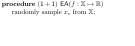
\includegraphics[width=0.75\paperwidth]{\sharedDir/graphics/metaheuristic_algorithms/opoea/opoea_2}}%
}{0.125}{0.445}%
%
\locate{4}{%
\algobox{0.75}{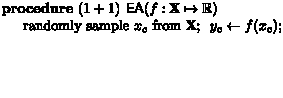
\includegraphics[width=0.75\paperwidth]{\sharedDir/graphics/metaheuristic_algorithms/opoea/opoea_3}}%
}{0.125}{0.445}%
%
\locate{5}{%
\algobox{0.75}{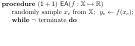
\includegraphics[width=0.75\paperwidth]{\sharedDir/graphics/metaheuristic_algorithms/opoea/opoea_4}}%
}{0.125}{0.445}%
%
\locate{6}{%
\algobox{0.75}{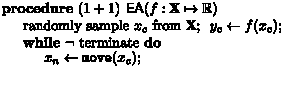
\includegraphics[width=0.75\paperwidth]{\sharedDir/graphics/metaheuristic_algorithms/opoea/opoea_5}}%
}{0.125}{0.445}%
%
\locate{7}{%
\algobox{0.75}{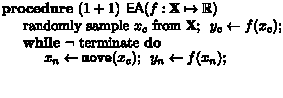
\includegraphics[width=0.75\paperwidth]{\sharedDir/graphics/metaheuristic_algorithms/opoea/opoea_6}}%
}{0.125}{0.445}%
%
\locate{8}{%
\algobox{0.75}{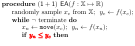
\includegraphics[width=0.75\paperwidth]{\sharedDir/graphics/metaheuristic_algorithms/opoea/opoea_7}}%
}{0.125}{0.445}%
%
\locate{9}{%
\algobox{0.75}{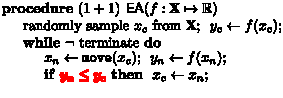
\includegraphics[width=0.75\paperwidth]{\sharedDir/graphics/metaheuristic_algorithms/opoea/opoea_8}}%
}{0.125}{0.445}%
%
\locate{10}{%
\algobox{0.75}{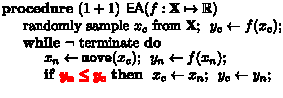
\includegraphics[width=0.75\paperwidth]{\sharedDir/graphics/metaheuristic_algorithms/opoea/opoea_9}}%
}{0.125}{0.445}%
%
\locate{11-}{%
\algobox{0.75}{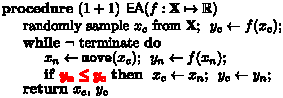
\includegraphics[width=0.75\paperwidth]{\sharedDir/graphics/metaheuristic_algorithms/opoea/opoea}}%
}{0.125}{0.445}%
%
\end{frame}%
%
\begin{frame}%
\frametitle{Simulated Annealing}%
\parbox{0.41\paperwidth}{%
\begin{itemize}%
\item \glsFull{algoSA}\cite{KGV1983OBSA} is a local search that accepts also worsening moves, but with a probability that decreases over time and with the difference in solution quality.%
\item<3-> ${\mathfrak{R}}_0^1$~be a random number uniformly distributed in~$[0,1)$.%
\item<6-> High temperatures~$T$ increase the acceptance probability~$P$ of worse solutions, low~$T$ reduce it.%
\item<7-> $P$~is regulated by temperature schedule with parameter\only<10->{s}~$T_0$\only<10->{ and~$\varepsilon$}.%
\end{itemize}%
}%
\uncover<11->{\begin{itemize}%
\item \gls{algoSA} also remembers best-so-far solution~$x_B$ and its objective value~$y_B$, because it could get lost.%
\end{itemize}%
}%
%
%
\locate{2}{%
\algobox{0.5}{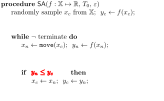
\includegraphics[width=0.5\paperwidth]{\sharedDir/graphics/metaheuristic_algorithms/sa/sa_01}}%
}{0.44}{0.24}%
%
\locate{3}{%
\algobox{0.5}{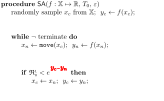
\includegraphics[width=0.5\paperwidth]{\sharedDir/graphics/metaheuristic_algorithms/sa/sa_02}}%
}{0.44}{0.24}%
%
\locate{4}{%
\algobox{0.4}{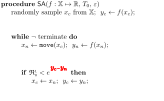
\includegraphics[width=0.4\paperwidth]{\sharedDir/graphics/metaheuristic_algorithms/sa/sa_02}}%
}{0.44}{0.07}%
%
\locate{4}{%
\resizebox{0.5\paperwidth}{!}{\bgroup%
\fboxsep=2pt%
\fboxrule=2pt%
\fcolorbox{black}{white}{%
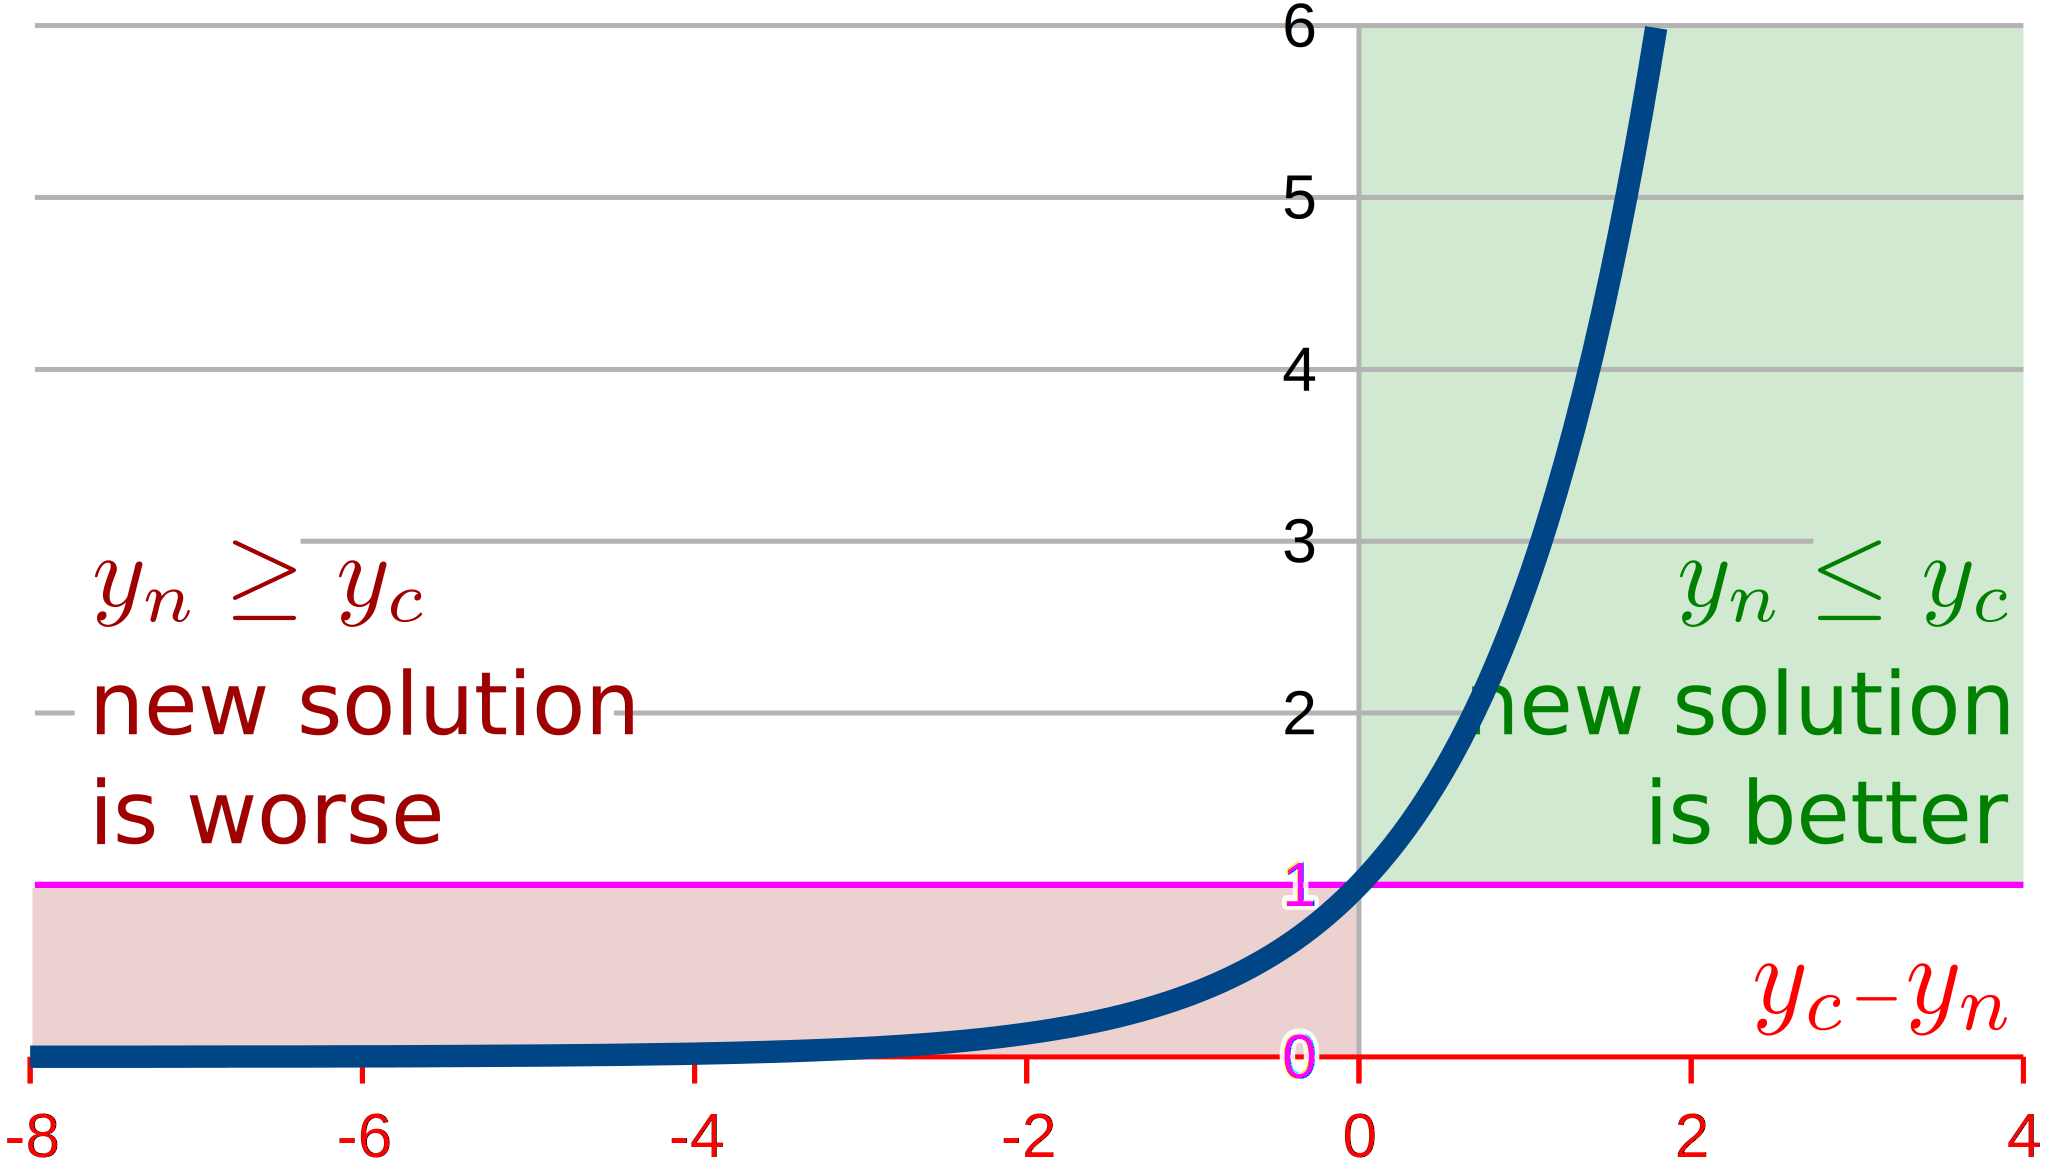
\includegraphics[width=0.5\paperwidth]{\sharedDir/graphics/metaheuristic_algorithms/sa/exp}%
}%
\egroup}%%
}{0.46}{0.41}%
%
\locate{5}{%
\algobox{0.5}{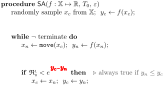
\includegraphics[width=0.5\paperwidth]{\sharedDir/graphics/metaheuristic_algorithms/sa/sa_03}}%
}{0.44}{0.24}%
%
\locate{6}{%
\algobox{0.5}{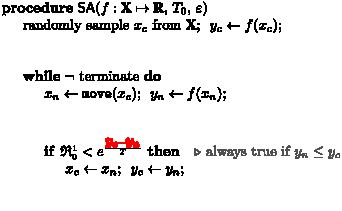
\includegraphics[width=0.5\paperwidth]{\sharedDir/graphics/metaheuristic_algorithms/sa/sa_04}}%
}{0.44}{0.24}%
%
\locate{7}{%
\algobox{0.5}{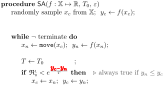
\includegraphics[width=0.5\paperwidth]{\sharedDir/graphics/metaheuristic_algorithms/sa/sa_05}}%
}{0.44}{0.24}%
%
\locate{8}{%
\algobox{0.5}{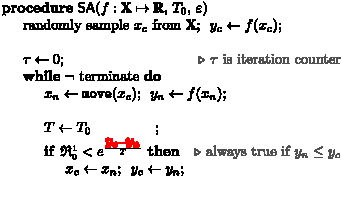
\includegraphics[width=0.5\paperwidth]{\sharedDir/graphics/metaheuristic_algorithms/sa/sa_06}}%
}{0.44}{0.24}%
%
\locate{9}{%
\algobox{0.5}{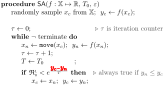
\includegraphics[width=0.5\paperwidth]{\sharedDir/graphics/metaheuristic_algorithms/sa/sa_07}}%
}{0.44}{0.24}%
%
\locate{10}{%
\algobox{0.5}{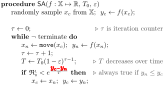
\includegraphics[width=0.5\paperwidth]{\sharedDir/graphics/metaheuristic_algorithms/sa/sa_08}}%
}{0.44}{0.24}%
%
\locate{11}{%
\algobox{0.5}{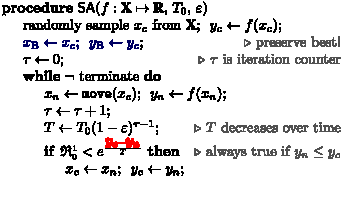
\includegraphics[width=0.5\paperwidth]{\sharedDir/graphics/metaheuristic_algorithms/sa/sa_09}}%
}{0.44}{0.24}%
%
\locate{12}{%
\algobox{0.5}{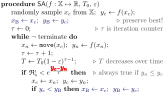
\includegraphics[width=0.5\paperwidth]{\sharedDir/graphics/metaheuristic_algorithms/sa/sa_10}}%
}{0.44}{0.24}%
%
\locate{13}{%
\algobox{0.5}{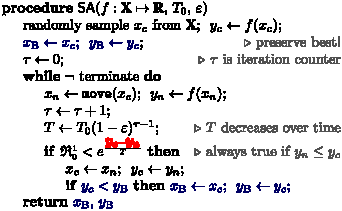
\includegraphics[width=0.5\paperwidth]{\sharedDir/graphics/metaheuristic_algorithms/sa/sa}}%
}{0.44}{0.24}%
%
\end{frame}%
%
\begin{frame}%
\frametitle{Standard Genetic Algorithm with Roulette Wheel Selection}%
\parbox{0.41\paperwidth}{%
\begin{itemize}%
\item The \glsFull{algoSGA} with Fitness Proportionate Selection~(Roulette Wheel) is for \textcolor{blue}{maximization}\cite{G1989GA,DJ2006ECAUA,W2009GOATAA,BFM1997HOEC,M1996GADSEP,M1998AITGA}.%
\item<2-> It uses a population of size~$ps$ as well as a unary\only<9->{ and binary} operator\only<9->{~(with crossover rate~$cr$)}.%
\end{itemize}%
}%
%
\locate{2}{%
\algobox{0.5}{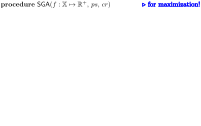
\includegraphics[width=0.5\paperwidth]{\sharedDir/graphics/metaheuristic_algorithms/sga/sga_01}}%
}{0.44}{0.24}%
%
\locate{3}{%
\algobox{0.5}{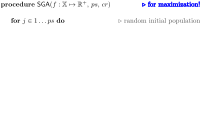
\includegraphics[width=0.5\paperwidth]{\sharedDir/graphics/metaheuristic_algorithms/sga/sga_02}}%
}{0.44}{0.24}%
%
\locate{4}{%
\algobox{0.5}{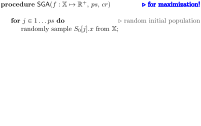
\includegraphics[width=0.5\paperwidth]{\sharedDir/graphics/metaheuristic_algorithms/sga/sga_03}}%
}{0.44}{0.24}%
%
\locate{5}{%
\algobox{0.5}{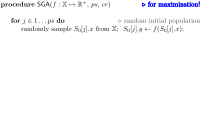
\includegraphics[width=0.5\paperwidth]{\sharedDir/graphics/metaheuristic_algorithms/sga/sga_04}}%
}{0.44}{0.24}%
%
\locate{6}{%
\algobox{0.5}{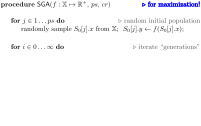
\includegraphics[width=0.5\paperwidth]{\sharedDir/graphics/metaheuristic_algorithms/sga/sga_05}}%
}{0.44}{0.24}%
%
\locate{7}{%
\algobox{0.5}{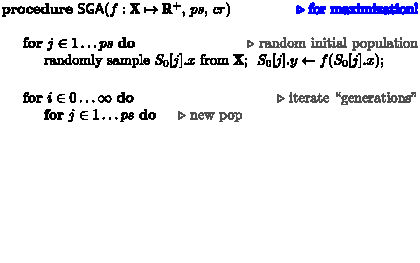
\includegraphics[width=0.5\paperwidth]{\sharedDir/graphics/metaheuristic_algorithms/sga/sga_06}}%
}{0.44}{0.24}%
%
\locate{8}{%
\algobox{0.5}{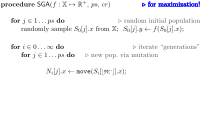
\includegraphics[width=0.5\paperwidth]{\sharedDir/graphics/metaheuristic_algorithms/sga/sga_07}}%
}{0.44}{0.24}%
%
\locate{9}{%
\algobox{0.5}{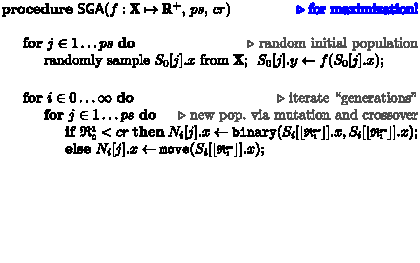
\includegraphics[width=0.5\paperwidth]{\sharedDir/graphics/metaheuristic_algorithms/sga/sga_08}}%
}{0.44}{0.24}%
%
\locate{10}{%
\algobox{0.5}{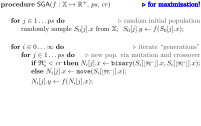
\includegraphics[width=0.5\paperwidth]{\sharedDir/graphics/metaheuristic_algorithms/sga/sga_09}}%
}{0.44}{0.24}%
%
\locate{11}{%
\algobox{0.5}{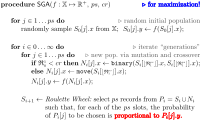
\includegraphics[width=0.5\paperwidth]{\sharedDir/graphics/metaheuristic_algorithms/sga/sga_10}}%
}{0.44}{0.24}%
%
\locate{12}{%
\algobox{0.5}{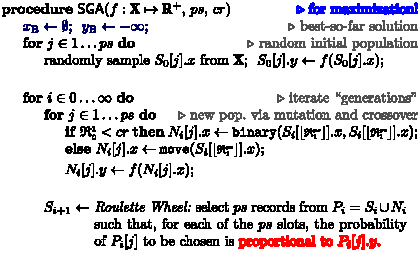
\includegraphics[width=0.5\paperwidth]{\sharedDir/graphics/metaheuristic_algorithms/sga/sga_11}}%
}{0.44}{0.24}%
%
\locate{13}{%
\algobox{0.5}{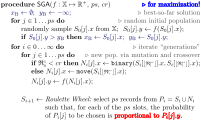
\includegraphics[width=0.5\paperwidth]{\sharedDir/graphics/metaheuristic_algorithms/sga/sga_12}}%
}{0.44}{0.24}%
%
\locate{14}{%
\algobox{0.5}{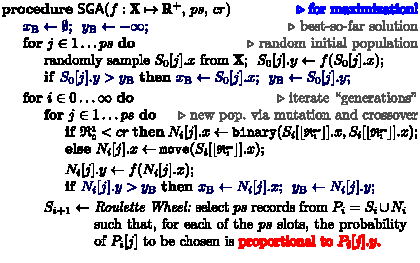
\includegraphics[width=0.5\paperwidth]{\sharedDir/graphics/metaheuristic_algorithms/sga/sga_13}}%
}{0.44}{0.24}%
%
\locate{15}{%
\algobox{0.5}{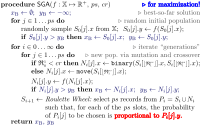
\includegraphics[width=0.5\paperwidth]{\sharedDir/graphics/metaheuristic_algorithms/sga/sga}}%
}{0.44}{0.24}%
%
\end{frame}%
%
\begin{frame}%
\frametitle{Metaheuristic Optimization}%
\begin{itemize}%
\item What we have learned is that different metaheuristics realize the trial-and-error scheme differently.%
\item<2-> During their selection steps, they all prefer better solutions over worse ones.%
\item<3-> If they would always and only accept the better solutions, they could get trapped in local optima.%
\item<4-> So some of them sometimes accept worse solutions, but the probability to choose a better solution is always higher in average.%
\item<5-> This is the most fundamental concept of metaheuristic optimization:%
\end{itemize}%
%
\uncover<5->{\smallskip%
\begin{center}\textbf{\large{\textcolor{red}{%
If you keep good solutions and modify them, you are likely to get better solutions.%
\uncover<6->{\medskip\\%
If you keep accepting better and better solutions, you will get really good solutions eventually.%
}%
}}}\end{center}%
}%
%
\end{frame}%
%
%
\section{Invariance Properties}%
%
\begin{frame}%
\frametitle{Invariance Properties}%
\begin{itemize}%
\item Research in optimization, \glsFull{ML}, and \glsFull{AI} often use simple problems to test and benchmark algorithms.%
\item<2-> These allow for many experiments in a short time.%
\item<3-> We often know the optimal solutions or at lower bounds for the optimal objective values.%
\item<4-> We can understand the results well.%
\item<5-> What we want is that algorithms perform similar to our benchmarking results also on actual, real-world problems.%
\item<6-> \alert{We want invariance properties.}\cite{OAAH2017IGOAAUPVIP,HA2014PDOCSSFTTP,JA2010LLCOTSIMMLEAOMFIRFLPS}%
\end{itemize}%
\end{frame}%
%
\begin{frame}%
\frametitle{Acceptance Criteria}%
\begin{itemize}%
\item We have now three example algorithms:~\gls{algoEAopo}, \gls{algoSA}, and \gls{algoSGA}.%
%
\item<2-> Assume that they all work on a population of two solutions, where the new solution be~$x_n$ and the old/parent solution be~$x_c$\only<3->{ and we look at the probability~$P$ to accept~$x_n$}.%
%
\item<4-> For the \gls{algoEAopo}, $P=1$ if~$f(x_n)\leq f(x_c)$ and~$0$~otherwise.%
%
\item<5-> In the \gls{algoSA}, $P$~depends on the difference~$\Delta=f(x_c)-f(x_n)$ and is~$1$~if $x_n$ is better than~$x_c$.%
%
\item<6-> In an \gls{algoSGA} for maximization, $P$~is~$f(x_n)/(f(x_c)+f(x_n))$.\uncover<7->{ If we wanted to do minimization, maybe we could use ${\color{orange}{1-}}f(x_n)/(f(x_c)+f(x_n))$ instead.}%
%
\item<8-> \gls{algoEAopo} and \gls{algoSA} always accept~$x_n$ if it is better than~$x_c$, while in the \gls{algoSGA}, a better~$x_n$ at least has a~$P>0.5$.%
%
\item<9-> Let's keep these things in mind.%
\end{itemize}%
\end{frame}%
%
\begin{frame}%
\frametitle{Invariance Properties: OneMax Example}%
\parbox{0.415\paperwidth}{%
\begin{itemize}%
\item OneMax is the simplest benchmark problem in discrete optimization\cite{M1992HGARWMAH}.%
\item<2-> It is defined over~$\searchSpace=\{0,1\}^n$, i.e., the bit strings of length~$n$.%
\item<3-> Goal:~\inQuotes{Find the bit string of all 1s!}%
\item<4-> \inQuotes{Maximize the number of 1s!}%
\item<5-> $\fn{1}(x)=n-\sum{x}$~(for minimization).%
\item<6-> Every reasonable algorithm can solve this problem.%
\end{itemize}%
}%
%
\locateGraphic{}{width=0.51\paperwidth}{\sharedDir/graphics/onemax/onemax_f1}{0.455}{0.27}%
%
\end{frame}%
%
%
\begin{frame}%
\frametitle{Invariance Properties: OneMax Example -- Translation}%
\parbox{0.415\paperwidth}{%
\begin{itemize}%
\item Now I create a slightly modified variant of this problem.%
\item<2-> $\fn{2}(x)=\fn{1}(x)+10$.%
\item<3-> Expectation: Any reasonable algorithm should perform the same on~$\fn{1}$ and~$\fn{2}$\only<-3>{.}\uncover<4->{, i.e., make the exact same decisions\only<5->{ given the same random seeds}.}%
%
\item<8-> $\fn{1}(x_n)=14$\uncover<9->{, $\fn{1}(x_c)=6$\uncover<10->{, $\fn{2}(x_n)=24$\uncover<11->{, $\fn{2}(x_c)=16$}}}%

\item<12-> \gls{algoEAopo}: $14\leq6$ \textcolor{greenYesColor}{$\mathbf{=}$} $24\leq16$ \greenYes%
%
\item<13-> \gls{algoSA}: $6-14$ \textcolor{greenYesColor}{$\mathbf{=}$} $16-24$ \greenYes%
%
\item<14-> \gls{algoSGA}: ${\color{orange}{1-}}14/(14+6)=0.3$ \textcolor{redNoColor}{$\mathbf{\neq}$} ${\color{orange}{1-}}24/(24+16)=0.4$ \redNo%
\end{itemize}%
}%
%
\locateGraphic{1}{width=0.51\paperwidth}{\sharedDir/graphics/onemax/onemax_f1}{0.455}{0.27}%
\locateGraphic{2-5}{width=0.51\paperwidth}{\sharedDir/graphics/onemax/onemax_f1_f2}{0.455}{0.27}%
\locateGraphic{6}{width=0.51\paperwidth}{\sharedDir/graphics/onemax/onemax_f1_f2_xcxn_1}{0.455}{0.27}%
\locateGraphic{7}{width=0.51\paperwidth}{\sharedDir/graphics/onemax/onemax_f1_f2_xcxn_2}{0.455}{0.27}%
\locateGraphic{8}{width=0.51\paperwidth}{\sharedDir/graphics/onemax/onemax_f1_f2_xcxn_3}{0.455}{0.27}%
\locateGraphic{9}{width=0.51\paperwidth}{\sharedDir/graphics/onemax/onemax_f1_f2_xcxn_4}{0.455}{0.27}%
\locateGraphic{10}{width=0.51\paperwidth}{\sharedDir/graphics/onemax/onemax_f1_f2_xcxn_5}{0.455}{0.27}%
\locateGraphic{11-}{width=0.51\paperwidth}{\sharedDir/graphics/onemax/onemax_f1_f2_xcxn_6}{0.455}{0.27}%
%
\locate{15-}{\algobox{0.6}{%
\parbox{0.6\paperwidth}{%
\begin{itemize}%
\item The \gls{algoEAopo} and \gls{algoSA} are invariant under translations of the objective function value.%
\item<16-> The \gls{algoSGA} is not, i.e., may give us different results for~$\fn{1}$ and~$\fn{2}$.%
\end{itemize}%
}}}{0.2}{0.3}%
%
\end{frame}%
%
%
\begin{frame}%
\frametitle{Invariance Properties: OneMax Example -- Scaling}%
\parbox{0.415\paperwidth}{%
\begin{itemize}%
\item Now I create another slightly modified variant of this problem.%
\item<2-> $\fn{3}(x)=0.8\fn{1}(x)$.%
\item<3-> Expectation: Any reasonable algorithm should perform the same on~$\fn{1}$ and~$\fn{3}$, i.e., make the exact same decisions given the same random seeds.%
%
\item<5-> $\fn{1}(x_n)=14$, $\fn{1}(x_c)=6$\uncover<6->{, $\fn{3}(x_n)=11.2$, $\fn{3}(x_c)=4.8$}%
%
\item<7-> \gls{algoEAopo}: $14\leq6$ \textcolor{greenYesColor}{$\mathbf{=}$} $11.2\leq4.8$ \greenYes%
%
\item<8-> \gls{algoSA}: $6-14$ \textcolor{redNoColor}{$\mathbf{\neq}$} $4.8-11.2$ \redNo%
%
\item<9-> \gls{algoSGA}: ${\color{orange}{1-}}14/(14+6)=0.3$ \textcolor{greenYesColor}{$\mathbf{=}$} ${\color{orange}{1-}}11.2/(11.2+4.8)=0.3$ \greenYes%
\end{itemize}%
}%
%
\locateGraphic{1}{width=0.51\paperwidth}{\sharedDir/graphics/onemax/onemax_f1_f2}{0.455}{0.27}%
\locateGraphic{2-3}{width=0.51\paperwidth}{\sharedDir/graphics/onemax/onemax_f1_f2_f3}{0.455}{0.27}%
\locateGraphic{4}{width=0.51\paperwidth}{\sharedDir/graphics/onemax/onemax_f1_f2_f3_xcxn_1}{0.455}{0.27}%
\locateGraphic{5}{width=0.51\paperwidth}{\sharedDir/graphics/onemax/onemax_f1_f2_f3_xcxn_2}{0.455}{0.27}%
\locateGraphic{6-}{width=0.51\paperwidth}{\sharedDir/graphics/onemax/onemax_f1_f2_f3_xcxn_3}{0.455}{0.27}%
%
\locate{10-}{\algobox{0.6}{%
\parbox{0.6\paperwidth}{%
\begin{itemize}%
\item The \gls{algoEAopo} and \gls{algoSGA} are invariant under scaling of the objective function value.%
\item<11-> \gls{algoSA} is not, i.e., may give us different results for~$\fn{1}$ and~$\fn{3}$.%
\end{itemize}%
}}}{0.2}{0.3}%
%
\end{frame}%
%
\begin{frame}%
\frametitle{Invariance Properties: OneMax Example -- Squaring}%
\parbox{0.415\paperwidth}{%
\begin{itemize}%
\item Now I create another slightly modified variant of this problem.%
\item<2-> $\fn{4}(x)=[\fn{1}(x)]^2$.%
\item<3-> Expectation: A nice algorithm should perform the same on~$\fn{1}$ and~$\fn{4}$, i.e., make the exact same decisions given the same random seeds.%
%
\item<4-> $\fn{1}(x_n)=14$, $\fn{1}(x_c)=6$\uncover<5->{, $\fn{4}(x_n)=196$, $\fn{4}(x_c)=36$}%
%
\item<6-> \gls{algoEAopo}: $14\leq6$ \textcolor{greenYesColor}{$\mathbf{=}$} $196\leq36$ \greenYes%
%
\item<7-> \gls{algoSA}: $6-14$ \textcolor{redNoColor}{$\mathbf{\neq}$} $36-196$ \redNo%
%
\item<8-> \gls{algoSGA}: ${\color{orange}{1-}}14/(14+6)=0.3$ \textcolor{redNoColor}{$\mathbf{\neq}$} ${\color{orange}{1-}}196/(196+36)\approx0.156$ \redNo%
\end{itemize}%
}%
%
\locateGraphic{1}{width=0.51\paperwidth}{\sharedDir/graphics/onemax/onemax_f1_f2_f3}{0.455}{0.27}%
\locateGraphic{2-3}{width=0.51\paperwidth}{\sharedDir/graphics/onemax/onemax_f1_f2_f3_f4}{0.455}{0.27}%
\locateGraphic{4-}{width=0.51\paperwidth}{\sharedDir/graphics/onemax/onemax_f1_f2_f3_f4_xcxn}{0.455}{0.27}%
%
\locate{9-}{\algobox{0.6}{%
\parbox{0.6\paperwidth}{%
\begin{itemize}%
\item The \gls{algoEAopo} is invariant under all order-preserving transformations of the objective function value.%
\item<10-> \gls{algoSA} and the \gls{algoSGA} are not, i.e., may give us different results for~$\fn{1}$ and~$\fn{4}$.%
\end{itemize}%
}}}{0.2}{0.3}%
%
\end{frame}%
%
\begin{frame}%
\centering%
\strut\\\strut\vfill\strut\\\strut%
{\large{Now let's enter eerie territory\dots}}%
\strut\\\strut\vfill\strut\\\strut%
\end{frame}%
%
\begin{frame}%
\frametitle{Invariance Properties: OneMax Example -- Trap}%
\parbox{0.415\paperwidth}{%
\begin{itemize}%
\item Now I create another modified variant of this problem:~a trap\cite{DJW2002OTAOTOPOEA,NB2003AAOTBOSEAOTF}.%
\item<2-> \mbox{$\fn{5}(x)=\left\{\begin{array}{rl}0&\textnormal{if~}\fn{1}(x)=50\\1+\fn{1}(x)&\textnormal{otherwise}\end{array}\right.$\hspace{-5em}}%
\item<4-> Expectation: Algorithm performance on~\fn{1} does not carry over to~\fn{5}.
\item<5-> Neither the \gls{algoEAopo}, \gls{algoSA}, nor the \gls{algoSGA} can deal with this well.%
\item<6-> The \gls{algoEAopo} has expected runtime~\bigThetab{n^n} on traps\cite{DJW2002OTAOTOPOEA}.%
\end{itemize}%
}%
\locateGraphic{1}{width=0.51\paperwidth}{\sharedDir/graphics/onemax/onemax_f1_f2_f3_f4}{0.455}{0.27}%
\locateGraphic{2}{width=0.51\paperwidth}{\sharedDir/graphics/onemax/onemax_f1_f5}{0.455}{0.27}%
\locateGraphic{3-}{width=0.51\paperwidth}{\sharedDir/graphics/onemax/onemax_f1_f5_optswap}{0.455}{0.27}%
\end{frame}%
%
\begin{frame}%
\frametitle{Invariance Properties: OneMax Example -- Jump}%
\parbox{0.415\paperwidth}{%
\begin{itemize}%
\item Now I create another modified variant of this problem:~a jump of width~$\omega=10$~bits.%
\item<2-> $\fn{6}(x)$ has a deceptive area of $\omega-1$ bits before the optimum.%
\item<3-> Expectation: Algorithm performance on~\fn{1} does not carry over to~\fn{6}.%
\item<4-> Neither the \gls{algoEAopo}, \gls{algoSA}, nor the \gls{algoSGA} can deal with this well.%
\item<5-> The \gls{algoEAopo} has expected runtime~\bigThetab{n^{\omega} + n\ln{n}} on jumps\cite{DJW2002OTAOTOPOEA}.%
\end{itemize}%
}%
\locateGraphic{}{width=0.51\paperwidth}{\sharedDir/graphics/onemax/onemax_f1_f6}{0.455}{0.27}%
\end{frame}%
%
\begin{frame}%
\frametitle{Invariance Properties: OneMax Example -- Injection}%
\parbox{0.415\paperwidth}{%
\begin{itemize}%
\item How about I apply an arbitrary injection~$g$ that preserves the location of optimum to~\fn{1} and get~$\fn{7}(x)=g(\fn{1}(x))$?.%
\item<2-> Expectation: Algorithm performance on~\fn{1} is probably unrelated to performance on~\fn{7}.%
\item<3-> Neither the \gls{algoEAopo}, \gls{algoSA}, nor the \gls{algoSGA} can deal with this well.%
\item<4-> Indeed, \alert{no} existing algorithm can deal with this, let alone have some invariance properties with respect to \emph{that}.%
\end{itemize}%
}%
\locateGraphic{}{width=0.51\paperwidth}{\sharedDir/graphics/onemax/onemax_f1_f7}{0.455}{0.27}%
\end{frame}%
%
\begin{frame}%
\uncover<-2>{%
Indeed, \alert{no} existing algorithm can deal with this, let alone have some invariance properties with respect to \emph{that}.%
\uncover<2->{%
\\\strut\\well\dots%
}}%
\locateGraphic{3}{width=0.6\paperwidth}{\sharedDir/graphics/papers/WWLC2021FFAMOAIUBTOTOFV}{0.2}{0.04}%
%
\locate{3}{\parbox{0.9\paperwidth}{%
\tiny{T Weise, Z Wu, X Li, and Y Chen. \citetitle{WWLC2021FFAMOAIUBTOTOFV}. IEEE Transactions on Evolutionary Computation~25(2):307–319. 2021.~\bracketCite{WWLC2021FFAMOAIUBTOTOFV}~{[copyright IEEE]}}%
}}{0.05}{0.91}%
%
\end{frame}%
%
\section{Frequency Fitness Assignment}%
%
\begin{frame}%
\frametitle{FFA: Idea}%
\begin{itemize}%
\item \GlsFull{algoFFA} is a module that can be plugged into different existing algorithms.%
\item<2-> It changes the way the algorithm selects the interesting solutions~$S_{i+1}$ from the sets~$P_i=S_i\cup N_i$.%
\item<3-> It therefore maintains a table~$H$ with the encounter frequency of each objective value in the selection decisions.%
\item<4-> The table~$H$ is initially filled with zeros.%
\item<5-> Before the selection step of the algorithm, $H[f(P_i[j])]$ for all $j\in\intRange{1}{|P_i|}$ is incremented by~1.%
\item<6-> Then, the frequencies~$H[f(P_i[j])]$ replace the objective values $f(P_i[j])$ in the actual selection decisions.%
\end{itemize}%
\end{frame}%
%
\begin{frame}[t]%
\frametitle{FFA: (1+1)~EA and (1+1)~FEA}%
%
\begin{itemize}%
\only<-1>{%
\item Let's plug \gls{algoFFA} into the \gls{algoEAopo} and obtain the \glsFull{algoFEAopo}.%
}%
\only<-2>{%
\item<2-> We start with the \gls{algoEAopo}.%
}\only<-3>{%
\item<3-> We begin by initializing the frequency table~$H$ with all zeros.%
}\only<-4>{%
\item<4-> \emph{Before} the selection decision, we increment the frequency values of the objective values of all current solutions.%
}\only<-5>{%
\item<5-> Now the frequency values replace the objective values in the selection decisions.%
}%
\item<6-> Since we may now lose the best-so-far solution, we need to track it in additional variables.%
\item<8-> {\dots}which are then the return values of the \gls{algoFEAopo}.%
\end{itemize}%
%
\locate{}{%
\algobox{0.45}{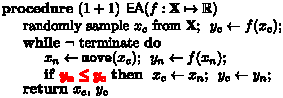
\includegraphics[width=0.45\paperwidth]{\sharedDir/graphics/metaheuristic_algorithms/opoea/opoea}}%
}{0.033333333}{0.4}%
%
%
\locate{2-}{%
\algobox{0.45}{%
\only<2>{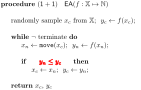
\includegraphics[width=0.45\paperwidth]{\sharedDir/graphics/metaheuristic_algorithms/fea/fea_1}}%
\only<3>{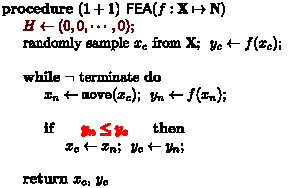
\includegraphics[width=0.45\paperwidth]{\sharedDir/graphics/metaheuristic_algorithms/fea/fea_2}}%
\only<4>{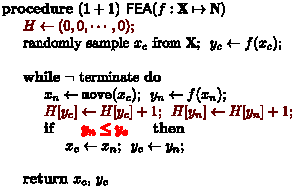
\includegraphics[width=0.45\paperwidth]{\sharedDir/graphics/metaheuristic_algorithms/fea/fea_3}}%
\only<5>{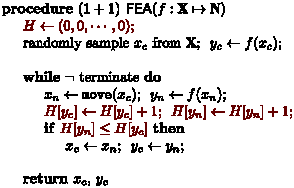
\includegraphics[width=0.45\paperwidth]{\sharedDir/graphics/metaheuristic_algorithms/fea/fea_4}}%
\only<6>{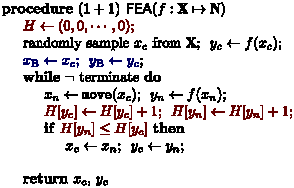
\includegraphics[width=0.45\paperwidth]{\sharedDir/graphics/metaheuristic_algorithms/fea/fea_5}}%
\only<7>{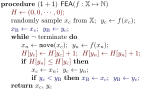
\includegraphics[width=0.45\paperwidth]{\sharedDir/graphics/metaheuristic_algorithms/fea/fea_6}}%
\only<8->{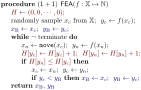
\includegraphics[width=0.45\paperwidth]{\sharedDir/graphics/metaheuristic_algorithms/fea/fea}}%
}%
}{0.516666666}{0.3}%
%
\end{frame}%
%
\begin{frame}%
\frametitle{FFA: What does this do?}%
\begin{itemize}%
\item The rating $H[f(x)]$ of a solution~$x$ depends only on the identity of~$f(x)$.
\item<2-> The rating $H[f(x)]$ of a solution~$x$ depends only on how often solutions~$x'$ with $f(x')=f(x)$ have previously been seen in the optimization process.%
\item<3-> Static optimization problems become dynamic, because frequency fitness~$H$ changes over time.%
\item<4-> Solutions get less attractive the more often their corresponding objective values have been seen. This also holds for local optima\dots%
\item<5-> Solutions with better objective values are no longer preferred over such with worse objective value.%
\item<6-> Instead, solutions with less-frequent objective values are preferred.%
\item<7-> \alert{Algorithms using \gls{algoFFA} are invariant under all injective transformations of the objective function value.}%
\item<8-> \alert{They perform identical on ALL of the OneMax-based functions from before!}%
\end{itemize}%
\end{frame}%
%
\begin{frame}[t]%
\frametitle{Discrete Optimization Theory Benchmarks}%
\begin{itemize}%
\item If we use the encounter frequency of objective values as \alert{only} guide for optimization {\dots} can this work?%
\item<2-> Why should this lead to anything but strange random walks?%
\item<3-> So we tested it on discrete optimization benchmarks.%
\end{itemize}%
%
\locateGraphic{3}{width=0.5\paperwidth}{\sharedDir/graphics/discrete_benchmarks/discrete_benchmarks}{0.25}{0.40}%
\end{frame}%
%
\begin{frame}%
\frametitle{(1+1)~FEA on OneMax}%
\parbox{0.37\paperwidth}{%
\begin{itemize}%
\item As first example, we again take OneMax\cite{M1992HGARWMAH}.%
\item<2-> The expected runtime of \gls{algoEAopo} on OneMax is in \bigThetab{n\ln{n}}.\cite{DDE2015FBBCTDNGA,M1992HGARWMAH}%
\item<3-> The average runtime \gls{algoFEAopo} on OneMax seems to be slower by factor proportional to~$n$, i.e., seems to be in~\bigOb{n^2\ln{n}}.%
\end{itemize}%
}%
%
\locateGraphic{}{width=0.55\paperwidth}{\sharedDir/graphics/fea_performance/fea_onemax}{0.41}{0.22}%
%
\end{frame}%
%
\begin{frame}%
\frametitle{(1+1)~FEA on LeadingOnes}%
\parbox{0.37\paperwidth}{%
\begin{itemize}%
\item The LeadingOnes problem maximizes the number of leading \texttt{1} bits in a bit string\cite{W1989TGAASPWRBAORTIB,R1997CPOEA}.%
\item<2-> The expected runtime of \gls{algoEAopo} on LeadingOnes is in \bigThetab{n^2}.\cite{DJW2002OTAOTOPOEA}%
\item<3-> The average runtime \gls{algoFEAopo} on LeadingOnes seems to be slower by factor proportional to~$n$, i.e., seems to be in~\bigOb{n^3}.%
\end{itemize}%
}%
%
\locateGraphic{}{width=0.55\paperwidth}{\sharedDir/graphics/fea_performance/fea_leadingones}{0.41}{0.22}%
%
\end{frame}%
%
\begin{frame}%
\frametitle{(1+1)~FEA on TwoMax}%
\parbox{0.37\paperwidth}{%
\begin{itemize}%
\item The TwoMax problem has one local opposite to a global optimum\cite{FQW2018ELDBOAWHTMO,VHGN2002FTTIMEAHSP}.%
\item<2-> An \gls{algoEAopo} has a 50/50 chance to converge to the local or global optimum and thus has an expected runtime in \bigThetab{n^n}.\cite{FQW2018ELDBOAWHTMO,FOSW2009AODPMFGE}%
\item<3-> The average runtime \gls{algoFEAopo} on TwoMax seems to be in~\bigOb{n^2 \ln{n}}.%
\end{itemize}%
}%
%
\locateGraphic{1}{width=0.55\paperwidth}{\sharedDir/graphics/discrete_benchmarks/discrete_benchmarks_twomax}{0.41}{0.22}%
\locateGraphic{2-}{width=0.55\paperwidth}{\sharedDir/graphics/fea_performance/fea_twomax}{0.41}{0.22}%
%
\end{frame}%
%
\begin{frame}%
\frametitle{(1+1)~FEA on Trap}%
\parbox{0.37\paperwidth}{%
\begin{itemize}%
\item The Trap problem basically swaps the global optimum with the worst solution\cite{DJW2002OTAOTOPOEA,NB2003AAOTBOSEAOTF}.%
\item<2-> An \gls{algoEAopo} will converge to the resulting local optimum and thus have an expected runtime of \bigThetab{n^n}.\cite{DJW2002OTAOTOPOEA}%
\item<3-> The average runtime \gls{algoFEAopo} on Trap seems to be in~\bigOb{n^2 \ln{n}}.%
\end{itemize}%
}\\%
\uncover<4->{\begin{itemize}%
\item The expected runtime is the same as on OneMax, because Trap is an injective transformation of OneMax, symmetric, and FFA \inQuotes{converges} into both directions.%
\end{itemize}%
}%
%
\locateGraphic{1}{width=0.55\paperwidth}{\sharedDir/graphics/discrete_benchmarks/discrete_benchmarks_onemax_trap}{0.41}{0.22}%
\locateGraphic{2-}{width=0.55\paperwidth}{\sharedDir/graphics/fea_performance/fea_trap}{0.41}{0.22}%
%
\end{frame}%
%
\begin{frame}%
\frametitle{(1+1)~FEA on Jumps}%
\parbox{0.37\paperwidth}{%
\begin{itemize}%
\item The Jump problem inserts a deceptive region of~$\omega-1$~bits before the optimum, forcing the algorithm to toggle~$\omega$ bits at once\cite{DJW2002OTAOTOPOEA,FQW2018ELDBOAWHTMO}.%
\item<2-> An \gls{algoEAopo} will converge to the resulting local optimum and thus have an expected runtime of \bigThetab{n^{\omega}+n\ln{n}}.\cite{DJW2002OTAOTOPOEA}%
\item<3-> The average runtime \gls{algoFEAopo} on Jump seems to \alert{always} be in~\bigOb{n^2 \ln{n}}.%
\end{itemize}%
}\\%
\uncover<4->{\begin{itemize}%
\item It is \alert{identical} to its performance on OneMax regardless of~$\omega$, because all Jumps are an injective transformation of OneMax!%
\end{itemize}%
}%
%
\locateGraphic{1}{width=0.55\paperwidth}{\sharedDir/graphics/discrete_benchmarks/discrete_benchmarks_jump}{0.41}{0.22}%
\locateGraphic{2-}{width=0.55\paperwidth}{\sharedDir/graphics/fea_performance/fea_jump}{0.41}{0.22}%
%
\end{frame}%
%
\begin{frame}%
\frametitle{(1+1)~FEA on Plateaus}%
\parbox{0.37\paperwidth}{%
\begin{itemize}%
\item The Plateau problem inserts a neutral region of~$\omega-1$~bits before the optimum, forcing the algorithm to toggle~$\omega$ bits at once\cite{AD2018PRAFP}.%
\item<2-> An \gls{algoEAopo} has an expected runtime of \bigThetab{n^{\omega}} on plateaus\cite{AD2018PRAFP}.%
\item<3-> The average runtime \gls{algoFEAopo} on Plateaus is slower, again by a factor seemingly proportional in~$n$.%
\item<4-> Plateaus remain plateaus under the identity-based fitness assignment FFA.%
\end{itemize}%
}%
%
\locateGraphic{1}{width=0.55\paperwidth}{\sharedDir/graphics/discrete_benchmarks/discrete_benchmarks_plateau}{0.41}{0.22}%
\locateGraphic{2-}{width=0.55\paperwidth}{\sharedDir/graphics/fea_performance/fea_plateau}{0.41}{0.22}%
%
\end{frame}%
%
\begin{frame}%
\frametitle{(1+1)~FEA on MaxSAT}%
\begin{itemize}%
\item The \glsFull{optMaxSAT}\cite{HS2004SLSFAA,C1971TCOTPP} problem is \npComplete~\cite{C1971TCOTPP}.%
\item<2-> \gls{SATLIB}\cite{HS2000SAORFROS} provides satisfiable benchmark instances from the phase transition region~(i.e., the hardest type of instances) for different scales~$n\in20 \cup \{25 i\; \forall i \in \intRange{2}{10}\}$.%
\item<3-> We conducted 11\decSep000~runs with the \gls{algoFEAopo} on each instance scale.%
\item<4-> The \gls{algoEAopo} is very much slower than the \gls{algoFEAopo}, so we could use it only on smaller scales.%
\item<5-> Our computational budget was always~$10^{10}$~\glsFullpl{objFE}.%
\end{itemize}%
%
\end{frame}%
%
\begin{frame}%
\frametitle{(1+1)~FEA on MaxSAT}%
\parbox{0.25\paperwidth}{%
\begin{itemize}%
\item The \gls{algoFEAopo} is better on problems with 250 variables than the \gls{algoEAopo} on problems with 50.%
\end{itemize}%
}%
%
\locateGraphic{}{width=0.65\paperwidth}{\sharedDir/graphics/fea_performance/fea_maxsat_table}{0.3}{0.22}%
%
\end{frame}%
%
\begin{frame}%
\frametitle{(1+1)~FEA on MaxSAT: ERT-ECDF}%
%
\locateGraphic[\citetitle{WWLC2021FFAMOAIUBTOTOFV}~\bracketCite{WWLC2021FFAMOAIUBTOTOFV}]{}{width=0.75\paperwidth}{\sharedDir/graphics/fea_performance/fea_maxsat_ecdf}{0.125}{0.15}%
%
\end{frame}%
%
\begin{frame}%
\frametitle{FFA: What does this do?}%
%
\begin{itemize}%
\item So it turns out, \gls{algoFFA} does work.%
\item<2-> It works because it prefers solutions with rare objective values.%
\item<3-> Solutions with very good objective values are also very rare on any problem worth tackling.%
\item<4-> FFA makes the simple \gls{algoEAopo} slower on problems that it can easily solve.%
\item<5-> The slowdown is roughly proportional to the number of possible different objective values.%
\item<6-> On some non-\npHard\ problems for which the \gls{algoEAopo} needs \alert{exponential} runtime, the \gls{algoFEAopo} needs \alert{polynomial} mean runtime.%
\item<7-> But not for all, because plateaus of the objective are still plateaus under \gls{algoFFA}.%
\item<8-> \gls{algoFFA} very significantly speeds up the \gls{algoEAopo} on the \npComplete\ \gls{optMaxSAT} problem.%
\end{itemize}%
%
\end{frame}%
%
\begin{frame}%
\frametitle{FFA: Let's get weird!}%
%
\only<-1>{\centering\strut\\\vfill\strut{\Large{Let's get weird!}}\strut\\\vfill\strut}%
%
\uncover<2->{%
\begin{itemize}%
\item Let’s say you have an optimization problem with objective function~$f(x)$.%
\item<3-> You \alert{encrypt} the objective values and do not tell them to the algorithm.%
\item<4-> Let's say you apply \glslink{cryptoAES}{AES}\cite{FIPSPUB197,FIPSPUB197upd1}, \gls{cryptoRSA}\cite{RSA1978AMFODSAPKC,Y2006MCFCTR}, or the Caesar cipher\cite{O2002CACJCTEATI,Y2006MCFCTR} as a function~$g:\naturalNumbersZ\mapsto\naturalNumbersZ$ to~$f$, i.e., do~$g\circ f$.%
\item<5-> Encryption removes any order, correlation or causality information, i.e., $g\circ f$ does not correlate with~$f$ in any way.%
\item<6-> $g(f(x))$~will be totally random.\uncover<7->{ No reasonable optimization algorithm could work with that.}%
\item<8-> If the \gls{algoFEAopo} can find the optimum of~$f(x)$\dots%
\item<9-> {\dots}then it will find exactly the same solution in exactly the same runtime even if you apply it to the encrypted problem~$g(f(x))$!%
\item<10-> How incredibly strange is that?%
\end{itemize}%
}%
%
\end{frame}%
%
%
\section{Where did we try FFA?}%
%
\begin{frame}%
\frametitle{Applications of FFA}%
\begin{itemize}%
\item Often, when some new type of algorithm is designed, one is tempted to pick some special, niche problems as application area.%
\item<2-> Then, the competition is not so high and it's easier to get some good papers out.%
\item<3-> We did not do this.%
\item<4-> We picked some of the most popular \npHard\ problems as testbeds.%
\item<5-> We could not (yet) win against the state-of-the-art that matured over decades.%
\item<6-> But we did get some interesting results on real, hard, and well-known problems.%
\end{itemize}%
\end{frame}%
%
\begin{frame}%
\frametitle{Maximum Satisfiability Problem}%
\begin{itemize}%
\item \Gls{algoFFA} on the \glsFull{optMaxSAT} Problem:~\bracketCite{WWLCL2023FFAOWBFGSCBE,WWLC2021FFAMOAIUBTOTOFV,WWWTDY2014FFA}.%
\end{itemize}%
%
\uncover<2->{%
\vspace{-1em}%
\begin{center}%
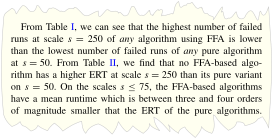
\includegraphics[width=0.6\paperwidth]{\sharedDir/graphics/papers/WWLCL2023FFAOWBFGSCBE_p10_snippet}%
\end{center}%
\vspace{-1em}%
%
\begin{itemize}%
\item Snippet of page~10 of~\bracketCite{WWLCL2023FFAOWBFGSCBE}~(copyright~IEEE).%
\item Several different \glspl{algoEA} with and without \gls{algoFFA}%
\item Budget:~$10^{10}$~\glspl{objFE}%
\end{itemize}%%
}%
%
\end{frame}%
%
\begin{frame}%
\frametitle{Traveling Salesperson Problem}%
\parbox{0.5\paperwidth}{%
\begin{itemize}%
\item \Gls{algoFFA} on the \glsFull{optTSP}:~\bracketCite{LWLvdBTW2024ATTSPWFFAAHA,LWLvdBW2022STTSPUFFA,LWTWW2024GSIWIFFTTSP}.%
\item<2-> Snippet of page~12 of~\bracketCite{LWLvdBTW2024ATTSPWFFAAHA}~(copyright Springer).%
\item<2-> \gls{algoEAopo}, \gls{algoFEAopo}, \gls{algoSA} w/o \gls{algoFFA}, hybrids%
\item<2-> Budget:~$10^{10}$~\glspl{objFE}%
\end{itemize}%
}%
%
\locateGraphic{2}{width=0.45\paperwidth}{\sharedDir/graphics/papers/LWLvdBTW2024ATTSPWFFAAHA_p12_snippet}{0.525}{0.03}%
\end{frame}%
%
\begin{frame}%
\frametitle{Quadratic Assignment Problem}%
\parbox{0.5\paperwidth}{%
\begin{itemize}%
\item \Gls{algoFFA} on the \glsFull{optQAP}:~\bracketCite{CWTW2024FFAOWBFGSORLSOTQAP,TOvdBLW2024ESTAEFFFA}.%
\item<2-> Snippet of page~7 of~\bracketCite{CWTW2024FFAOWBFGSORLSOTQAP}~(copyright SciTePress).%
\item<2-> \gls{algoRLS} w/o \gls{algoFFA}%
\item<2-> Budget:~$10^{8}$~\glspl{objFE}%
\end{itemize}%
}%
%
\locateGraphic{2}{width=0.45\paperwidth}{\sharedDir/graphics/papers/CWTW2024FFAOWBFGSORLSOTQAP_p7_snippet}{0.525}{0.03}%
%
\end{frame}%
%
\begin{frame}%
\frametitle{Job Shop Scheduling Problem}%
\begin{itemize}%
\item \Gls{algoFFA} on the \glsFull{optJSSP} Problem:~\bracketCite{WWLC2021FFAMOAIUBTOTOFV,WLCW2021SJSSPWUABFGS,dBTvdB2023FFAOJACR}.%
\end{itemize}%
%
\uncover<2->{%
\vspace{-1em}%
\begin{center}%
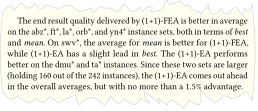
\includegraphics[width=0.6\paperwidth]{\sharedDir/graphics/papers/WLCW2021SJSSPWUABFGS_p4_snippet}%
\end{center}%
\vspace{-1em}%
%
\begin{itemize}%
\item Snippet of page~10 of~\bracketCite{WLCW2021SJSSPWUABFGS}~(copyright~ACM).%
\item Budget:~$2^{30}\approx10^{9}$~\glspl{objFE}%
\end{itemize}%%
}%
%
\end{frame}%
%
\begin{frame}%
\frametitle{Algorithm Synthesis and Genetic Programming}%
\begin{itemize}%
\item \Gls{algoFFA} for algorithm synthesis and \glsFull{algoGP}:~\bracketCite{WWTY2014EEIAWGP,WWWTDY2014FFA}.%
\end{itemize}%
%
\uncover<2->{%
\vspace{-1em}%
\begin{center}%
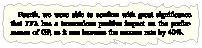
\includegraphics[width=0.6\paperwidth]{\sharedDir/graphics/papers/WWTY2014EEIAWGP_07_snippet}%
\end{center}%
\vspace{-1em}%
%
\begin{itemize}%
\item Snippet of page~7 of~\bracketCite{WWTY2014EEIAWGP}~(copyright~IEEE).%
\item Budget:~$\approx 100\decSep000$~\glspl{objFE}%
\end{itemize}%%
}%
%
\end{frame}%
%
\begin{frame}%
\frametitle{Where FFA did not work}%
\begin{itemize}%
\item \Gls{algoFFA} cannot work well on problems where local search already gives good results.%
\item<2-> This includes, surprisingly, also some computationally hard problems\only<-2>{.}\uncover<3->{:%
\begin{itemize}%
\item the \glsFull{optTTP}, where \gls{algoRLS} can find surprisingly good results:~\bracketCite{XWvdBW2024RLSVNVFFAOTTTP}.%
\item<4-> the two-dimensional bin packing problem, where \gls{algoRLS} can actually \alert{outperform} several complex state-of-the-art metaheuristics~\bracketCite{ZLWvdBTW2024RLSOT2RBPPWIR,ZWvdBTLTW2024RLSFTDBPAANRFFFA}.%
\end{itemize}%
}%
\end{itemize}%
\end{frame}%
%
\section{Summary}%
%
\begin{frame}%
\frametitle{Summary}%
\begin{itemize}%
\item \glsFull{algoFFA} is an algorithm module that can be plugged into existing algorithms.%
\item<2-> It renders algorithms invariant under all injective transformations of the objective function value.%
\item<3-> It makes them optimize without bias for good solutions.%
\item<4-> It slows them down on easy problems.%
\item<5-> It can speed them up on hard problems or lead them to solution qualities they otherwise cannot reach.%
\item<6-> It is limited to objective functions that cannot take on too many different objective values.%
\end{itemize}%
\end{frame}%
%
\section{Advertisement}%
%
\begin{frame}[t]%
\frametitle{Programming with Python}%
We have a freely available course book on \citetitle{programmingWithPython} at \citeurl{programmingWithPython}, with focus on practical software development using the \python\ ecosystem of tools\cite{programmingWithPython}.%
%
\locateGraphic{}{width=0.63\paperwidth}{\sharedDir/graphics/advertisement/snippets/programmingWithPythonSnippet}{0.025}{0.3}%
\locateGraphic{}{width=0.27\paperwidth}{\sharedDir/graphics/advertisement/urlQr/programmingWithPythonCourseUrl}{0.675}{0.4}%
%
\end{frame}%
%
\begin{frame}[t]%
\frametitle{Databases}%
We have a freely available course book on \citetitle{databases} at \citeurl{databases}, with actual practical examples using a real \dbms\cite{databases}.%
%
\locateGraphic{}{width=0.63\paperwidth}{\sharedDir/graphics/advertisement/snippets/databasesSnippet}{0.025}{0.3}%
\locateGraphic{}{width=0.27\paperwidth}{\sharedDir/graphics/advertisement/urlQr/databasesCourseUrl}{0.675}{0.4}%
%
\end{frame}%
%
%
\endPresentation%
\end{document}%%
\endinput%
%
